% ============================================================================
%  La biblioteca: buscar en los documentos y citar
%  Asesoría del proyecto final · Razonamiento Automático (prof. Fabián Serrano)
%  UNAL Manizales · Semana 2 · 80 min virtual
%  Mismo formato de las charlas: Beamer Boadilla 4:3, pdflatex (dos veces).
%  Manual: Manual_Semana2.tex
% ============================================================================
\documentclass[10pt]{beamer}
\usetheme{Boadilla}
\usecolortheme{default}
\usepackage[utf8]{inputenc}
\usepackage[T1]{fontenc}
\IfFileExists{spanish.ldf}
  {\usepackage[spanish,es-noshorthands]{babel}}
  {\usepackage[provide=*]{babel}\babelprovide[import=es, main]{spanish}}
\usepackage{xcolor}
\usepackage{listings}
\usepackage{graphicx}
\usepackage{booktabs}
\usepackage{amsmath}
\usepackage{amssymb}
\usepackage{stmaryrd}
\usepackage{alltt}
\setbeamertemplate{navigation symbols}{}
\setbeamertemplate{caption}[numbered]
\setbeamertemplate{blocks}[rounded][shadow=true]
\setbeamertemplate{itemize items}[circle]

\definecolor{psKey}{RGB}{0,80,160}
\definecolor{psCom}{RGB}{120,120,120}
\definecolor{psStr}{RGB}{160,60,0}
\definecolor{resalte}{RGB}{180,0,60}
\definecolor{confiable}{RGB}{0,120,60}
\setbeamercolor{alerted text}{fg=resalte}

\newcommand{\apuesta}[1]{%
  \begin{center}\large\color{resalte}\textbf{#1}\end{center}}
\newcommand{\clave}[1]{\textcolor{psKey}{#1}}
\newcommand{\carlos}[1]{\textcolor{red}{[[ #1 ]]}}

\usepackage{tikz}
\usetikzlibrary{arrows.meta,positioning,calc}

% --- Isabelle en alltt (como lo muestra jEdit) ---
\newcommand{\sImp}{\(\longrightarrow\)}
\newcommand{\kw}[1]{\textcolor{psKey}{\textbf{#1}}}
\newcommand{\str}[1]{\textcolor{psStr}{#1}}
\newcommand{\R}[1]{{\setlength{\fboxsep}{1pt}%
  \colorbox{resalte!12}{\ttfamily\bfseries\textcolor{resalte}{#1}}}}
\newcommand{\nota}[1]{{\small\itshape\color{psCom} #1}}
\newcommand{\cd}[1]{\texttt{#1}}
% colores usados por los diagramas
\colorlet{azul}{psKey}\colorlet{verde}{confiable}\colorlet{granate}{resalte}

% --- Python y terminal en listings ---
\lstset{basicstyle=\ttfamily\footnotesize, columns=fullflexible,
  keepspaces=true, showstringspaces=false, breaklines=true,
  keywordstyle=\color{psKey}\bfseries, commentstyle=\color{psCom}\itshape,
  stringstyle=\color{psStr},
  backgroundcolor=\color{black!5}, frame=leftline, rulecolor=\color{psKey!40},
  framesep=6pt, xleftmargin=8pt, aboveskip=0.4em, belowskip=0.4em}

\title[Semana 2: La biblioteca]{La biblioteca: buscar en los documentos y citar}
\subtitle{Asesoría del proyecto final --- Semana 2}
\author{Carlos Orrego}
\institute[UNAL]{Razonamiento Automático --- Prof.\ Fabián Serrano \\ Universidad Nacional de Colombia --- Sede Manizales}
\date{12 de noviembre de 2026}

\begin{document}

\maketitle

\begin{frame}{Hoy, en una frase}
  \vspace{1em}
  \begin{block}{Al salir de esta clase\ldots}
    \large
    \ldots el modelo ya no responde de memoria: antes de cada pregunta
    busca en los documentos del curso, y cita lo que usó.
  \end{block}
  \vspace{0.5em}
  \nota{Es la configuración 2: el mismo modelo de la semana pasada, con
  libro abierto.}
\end{frame}

\begin{frame}{Recorrido}
  \begin{center}
  \begin{tabular}{@{}rl@{}}
    \toprule
    Minutos & Parte \\
    \midrule
    0--10  & 1. La tarea: ¿cuánto dio la línea base? \\
    10--20 & 2. Examen a libro abierto \\
    20--40 & 3. Las piezas: normalizar, fragmentar, BM25 \\
    40--50 & 4. Medir la búsqueda sin gastar el modelo \\
    50--70 & 5. Taller: configuración 2 y citas \\
    70--80 & 6. Tarea \\
    \bottomrule
  \end{tabular}
  \end{center}
\end{frame}

\begin{frame}{Los cuatro jueves}
  \begin{center}
  \begin{tabular}{@{}lll@{}}
    \toprule
    Jueves & Nombre & Construimos \\
    \midrule
    1 & El hilo & el modelo y la línea base \\
    \alert{2 (hoy)} & \alert{La biblioteca} & \alert{buscar en los documentos y citar} \\
    3 & La flecha roja & verificar con Isabelle y corregir \\
    4 & El espejo & evaluar, analizar errores, informe \\
    \bottomrule
  \end{tabular}
  \end{center}
\end{frame}

% =====================================================================
\section{La tarea}

\begin{frame}{¿Cuánto dio su línea base?}
  \begin{itemize}
    \item Configuración 1 sobre las 58: ¿cuántas \cd{aceptada}, \cd{estilo},
      \cd{rechazada}, \cd{trampa}?
    \item De los diez registros que leyeron: ¿qué errores se repiten?
    \item ¿Qué tema de formalización eligió cada uno?
  \end{itemize}
  \vspace{0.6em}
  \nota{Ese número es contra el que se mide todo lo que hagamos hoy.}
\end{frame}

% =====================================================================
\section{Examen a libro abierto}

\begin{frame}{El modelo pequeño recuerda poco}
  \begin{itemize}
    \item La semana pasada vimos a Gemma inventar \cd{module Main},
      \cd{assert} y reglas \cd{and}, \cd{or}.
    \item No es falta de inteligencia: Isabelle es un rincón pequeño de lo
      que el modelo leyó.
    \item Pero el curso tiene \alert{588 lemas resueltos}, los dos libros de
      Alonso y las diapositivas.
  \end{itemize}
  \apuesta{¿Y si le damos el libro abierto en la página correcta?}
\end{frame}

\begin{frame}{La configuración 2}
  \begin{center}
  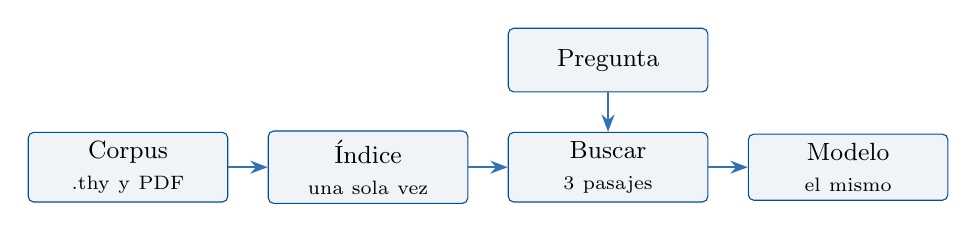
\begin{tikzpicture}[
      caja/.style={draw=azul, fill=azul!6, rounded corners=2pt,
                   minimum height=2.3em, align=center, font=\small, text width=2.3cm},
      flecha/.style={-{Stealth[length=2.2mm]}, thick, azul!80},
      node distance=0.5cm]
    \node[caja] (c) {Corpus\\{\scriptsize .thy y PDF}};
    \node[caja, right=of c] (i) {Índice\\{\scriptsize una sola vez}};
    \node[caja, right=of i] (b) {Buscar\\{\scriptsize 3 pasajes}};
    \node[caja, right=of b] (m) {Modelo\\{\scriptsize el mismo}};
    \node[caja, above=of b] (p) {Pregunta};
    \draw[flecha] (c) -- (i); \draw[flecha] (i) -- (b);
    \draw[flecha] (p) -- (b); \draw[flecha] (b) -- (m);
  \end{tikzpicture}
  \end{center}
  \begin{itemize}
    \item Todavía \alert{sin} Isabelle dentro del asistente: eso es el
      jueves 3.
    \item Mismo modelo y misma temperatura que la configuración 1. Si no,
      la comparación no mide la búsqueda.
  \end{itemize}
\end{frame}

% =====================================================================
\section{Las piezas}

\begin{frame}[fragile]{Pieza 1: normalizar los símbolos}
  En el \cd{.thy} dice \cd{\textbackslash<and>}; en el PDF y en el modelo,
  $\wedge$. Para la búsqueda deben ser la misma palabra.
\begin{lstlisting}[language=Python]
SIMBOLOS = {
    "and":     ["\\<and>", "∧"],
    "implies": ["\\<longrightarrow>", "⟶", "-->"],
    "entails": ["\\<Longrightarrow>", "⟹", "==>", "\\<turnstile>"],
    ...
}
\end{lstlisting}
  \nota{\cd{normalizar.py}. Se aplica al indexar \emph{y} al buscar.}
\end{frame}

\begin{frame}{Pieza 2: fragmentar por comandos, no por tamaño}
  \begin{itemize}
    \item Un fragmento empieza en un comando: \cd{lemma}, \cd{fun},
      \cd{definition}, \cd{section}\ldots
    \item Guarda archivo, línea y nombre: con eso se cita.
    \item El \cd{text} de antes \alert{se pega al lema}: ahí dice
      «Ejercicio 3. Demostrar \ldots».
    \item Un lema que termina en \cd{oops} no trae demostración: para
      demostrar no sirve.
    \item Los PDF, por página.
  \end{itemize}
  \vspace{0.4em}
  \nota{Resultado: 2\,318 fragmentos, 588 lemas con demostración, en 3
  segundos.}
\end{frame}

\begin{frame}{Pieza 3: BM25}
  Para cada fragmento, cada palabra de la consulta que aparece en él suma
  puntos. Suma más si:
  \begin{itemize}
    \item aparece varias veces, con techo;
    \item es \alert{rara} en el corpus: \cd{conjE} pesa más que \cd{by};
    \item el fragmento es corto.
  \end{itemize}
  \vspace{0.4em}
  \begin{block}{¿Por qué no \emph{embeddings}?}
    Las consultas importantes son literales: una regla, una función, una
    fórmula. BM25 son 30 líneas de Python sin descargar nada, y se explica
    completo en la sustentación.
  \end{block}
\end{frame}

% =====================================================================
\section{Medir la búsqueda}

\begin{frame}{Primero medir la búsqueda, después el modelo}
  \begin{itemize}
    \item Si la búsqueda no encuentra el pasaje, el modelo no tiene con qué
      mejorar, y uno culpa al modelo.
    \item En R1 se puede medir sin modelo: la solución del ejercicio $n$ es
      \cd{ejercicio\_n\_1} en \cd{R1\_Deduccion\_natural.thy}.
    \item \cd{medir\_recuperacion.py} cuenta en qué puesto queda.
  \end{itemize}
  \vspace{0.6em}
  \begin{center}
  \begin{tabular}{@{}lcc@{}}
    \toprule
    & primera & entre las 3 primeras \\
    \midrule
    Palabras sueltas & 3/58 & 15/58 \\
    \bottomrule
  \end{tabular}
  \end{center}
  \apuesta{¿Por qué tan mal?}
\end{frame}

\begin{frame}[fragile]{$p \longrightarrow q$ y $q \longrightarrow p$ son idénticas}
  Con palabras sueltas, las dos son \{\cd{p}, \cd{q}, \cd{implies}\}. En
  lógica proposicional todas las fórmulas usan las mismas palabras.

  \vspace{0.4em}
  El arreglo es una línea: contar también los \alert{pares de palabras
  seguidas}.
\begin{lstlisting}[language=Python]
def tokens(texto):
    t = re.findall(r"[a-z_][a-z0-9_']*|[0-9]+", normalizar(texto))
    return t + [a + "+" + b for a, b in zip(t, t[1:])]
\end{lstlisting}
  \begin{center}
  \begin{tabular}{@{}lcc@{}}
    \toprule
    & primera & entre las 3 primeras \\
    \midrule
    Palabras sueltas & 3/58 & 15/58 \\
    \alert{Con pares} & \alert{57/58} & \alert{58/58} \\
    Con pares, sin el número del ejercicio & 41/58 & 56/58 \\
    \bottomrule
  \end{tabular}
  \end{center}
  \nota{La última fila es la honesta: en el benchmark privado no habrá
  «Ejercicio 3» que coincida.}
\end{frame}

% =====================================================================
\section{Taller}

\begin{frame}[fragile]{Paso 1: traer y construir el índice}
\begin{lstlisting}[language=bash]
cd repo_proyecto_final
git pull
cd semana2/taller
python3 indexar.py
python3 buscar.py "conjE"
python3 medir_recuperacion.py
\end{lstlisting}
  \nota{Para los PDF: \cd{pip install pypdf} o \cd{brew install poppler}.
  Sin ellos se indexan solo las teorías, y para hoy basta.}
\end{frame}

\begin{frame}[fragile]{Paso 2: lo que recibe el modelo}
\begin{lstlisting}
Fragmentos del corpus del curso que pueden servir...

[F1] (TeoriasIsabelle/R1_Deduccion_natural.thy, linea 55 (ejercicio_1_1))
text \<open> Ejercicio 1. Demostrar ... \<close>
lemma ejercicio_1_1:
  assumes 1: "p \<longrightarrow> q" and 2: "p"
  shows "q"
proof - ...

[F2] ...   [F3] ...

Enunciado:
lemma ejercicio_1: ...
\end{lstlisting}
  \nota{3 fragmentos, cada uno cortado en 1\,500 caracteres: unos 4\,700 en
  total.}
\end{frame}

\begin{frame}{Un error nuevo: el modelo copia el fragmento}
  \begin{itemize}
    \item Con libro abierto, el modelo copia: el \cd{text}, la línea
      \cd{lemma ejercicio\_1\_1:} y a veces el lema siguiente.
    \item Para \cd{evaluar.py} eso es \alert{trampa}: trae \cd{lemma}.
    \item \cd{limpiar.py}: desde la primera palabra que abre una prueba
      (\cd{proof}, \cd{by}, \cd{using}\ldots) hasta el siguiente comando.
      Si no hay ninguna, vacío.
  \end{itemize}
  \vspace{0.4em}
  \nota{Lo encontramos con un modelo falso que copiaba el primer fragmento.
  Probar las tuberías con un modelo falso es barato y encuentra errores
  así.}
\end{frame}

\begin{frame}[fragile]{Paso 3: correr y calificar}
\begin{lstlisting}[language=bash]
python3 config2.py 3            # primero 3
python3 config2.py              # las 58
python3 ../../Recursos/evaluar.py ../../Recursos/benchmark_R1.json \
        respuestas_config2.json --paralelo 4 --informe informe_c2.json
\end{lstlisting}
  \begin{itemize}
    \item Usa el \cd{modelo.py} de la semana 1: el mismo modelo.
    \item \cd{registros/config2.jsonl} guarda también los pasajes y su
      puntaje (R5).
  \end{itemize}
\end{frame}


\begin{frame}{Lo que pasó en el ensayo: \texttt{llama3.2:3b}, 20 preguntas}
  \begin{center}
  \begin{tabular}{@{}lccc@{}}
    \toprule
    & aceptadas & rechazadas & trampa \\
    \midrule
    Configuración 1 (sin búsqueda) & 3 & 16 & 1 \\
    \alert{Configuración 2 (con búsqueda)} & \alert{9} & \alert{11} & \alert{0} \\
    \bottomrule
  \end{tabular}
  \end{center}
  \begin{itemize}
    \item El mismo modelo, con libro abierto, \alert{triplica} lo que Isabelle acepta.
    \item Sin búsqueda, en la pregunta 6 el modelo no paraba de escribir.
      Con los pasajes, terminó.
    \item Pero la búsqueda no es gratis: las preguntas 13, 14 y 15 pasaban
      sin ayuda y \alert{fallaron} con ella.
    \item En la 1, el modelo tenía la solución exacta en [F1] y la copió mal:
      escribió \cd{proof} donde el libro dice \cd{proof -}.
  \end{itemize}
  \nota{Tener el pasaje correcto no basta. El jueves 3, Isabelle le devuelve
  el error y el modelo corrige.}
\end{frame}


\begin{frame}[fragile]{Paso 4: preguntas con citas}
\begin{lstlisting}[language=bash]
python3 preguntar.py "Que diferencia hay entre rule y erule?"
\end{lstlisting}
  \begin{itemize}
    \item El modelo cita \alert{por etiqueta}: [F2].
    \item El programa traduce la etiqueta en archivo y línea, o documento y
      página. El modelo no escribe rutas.
    \item Si usa una etiqueta que no existe: \cd{!! CITA INVENTADA}.
  \end{itemize}
  \vspace{0.4em}
  \nota{Que la etiqueta exista no garantiza que el fragmento diga eso. Eso
  se revisa a mano.}
\end{frame}

% =====================================================================
\section{Tarea}

\begin{frame}{Tarea para el jueves 3}
  \begin{enumerate}
    \item Índice construido y \cd{medir\_recuperacion.py} corrido.
    \item Configuración 2 sobre las 58, mismo modelo, calificada. ¿Cuánto
      subió? ¿Cuántas \cd{estilo}?
    \item Preguntas del anexo A con \cd{preguntar.py}, y cada cita revisada
      a mano.
    \item Tres preguntas trampa: premisa falsa, fuera de tema, y una que el
      corpus no responde.
    \item Formalización: cinco enunciados escritos. Indexen sus soluciones
      y midan si la búsqueda las encuentra.
  \end{enumerate}
\end{frame}

\begin{frame}{El jueves 3: la flecha roja}
  \vspace{1em}
  \centering
  \Large
  Hoy el modelo lee antes de escribir.\\[0.5em]
  El jueves, Isabelle le devuelve el error\\
  y el modelo \alert{corrige}.
\end{frame}

\end{document}
